\clearpage{\pagestyle{empty}\cleardoublepage}
\chapter{Applicazioni di schiumogeno per l'ottimizzazione della produzione degli idrocarburi}
\chaptermark{Applicazioni di schiumogeno}
Per \textit{Gas Well Deliquification} o \textit{Gas Well Dewatering} (GWD) si intende l'insieme delle tecnologie e delle applicazioni utili alla rimozione di acqua o condensati in fase produttiva da un pozzo a gas. Nello specifico il concetto di GDW racchiude tutti gli strumenti utili nel combattere il fenomeno del \textit{liquid loading}, definito come l'accumulo di acqua in pozzo e l'impossibilità di rimuoverla. Le tecnologie impiegate per lo spiazzamento dei liquidi a fondo pozzo sono numerose e sono in continua evoluzione per garantire migliori performance e affidabilità. Nell'ultimo decennio gli schiumogeni sembrano rappresentare una scelta concreta per controllare il carico idrostatico di fondo pozzo e presentano notevoli vantaggi rispetto alle tecnologie già esistenti \parencite{stanculescu2014gwd}. In questo capitolo sono descritte le cause e le conseguenze del \textit{liquid loading} e le principali tecnologie impiegate oggi per la riduzione e controllo del battente idrostatico. Particolare attenzione è dedicata all'impiego di tensioattivi liquidi o \textit{foamer}, descrivendo le proprietà fisico-chimiche, le procedure operative per il loro impiego e controllo tramite l'uso di antischiuma o  \textit{defoamer}.

\section{Liquid loading}
\subsection{Ciclo di vita di un pozzo a gas}
Nel paragrafo \ref{sssec:verticali} si è discusso dei diversi regimi di flusso bifase per condotte verticali. Un pozzo a gas può presentare tutti i regimi di flusso: in \figref{fig:declinecurve} è possibile comprendere graficamente l'evoluzione del pozzo durante il suo ciclo di vita. La distribuzione delle varie fasi in pozzo si evolve nel coso della vita produttiva. Inizialmente il gas è fase dominante e il pozzo ha forza sufficiente per trascinare tutto il liquido presente sul fondo. Ad alte velocità superficiali del gas corrisponde un regime anulare misto: la fase liquida è interdispersa nella fase gassosa. Con il diminuire della velocità del gas nel tempo, la fase liquida comincia a precipitare e a depositarsi sul fondo, ostacolando la normale produzione di gas.

\subsection{Problemi legati al liquid loading}
Il liquid loading porta a un regime di flusso a slug e a una produzione di gas discontinua e inferiore. Se il gas ha energia sufficiente a rimuovere i liquidi presenti a fondo pozzo, la portata del gas risponde in modo corretto alla stima di produzione rispetto al tempo di vita del pozzo, definita tramite l'analisi della curva di declino (\textit{Decline Curve Analysis}, DCA), visibile sempre in \figref{fig:declinecurve}.

\begin{figure}[htbp]
    \centering
    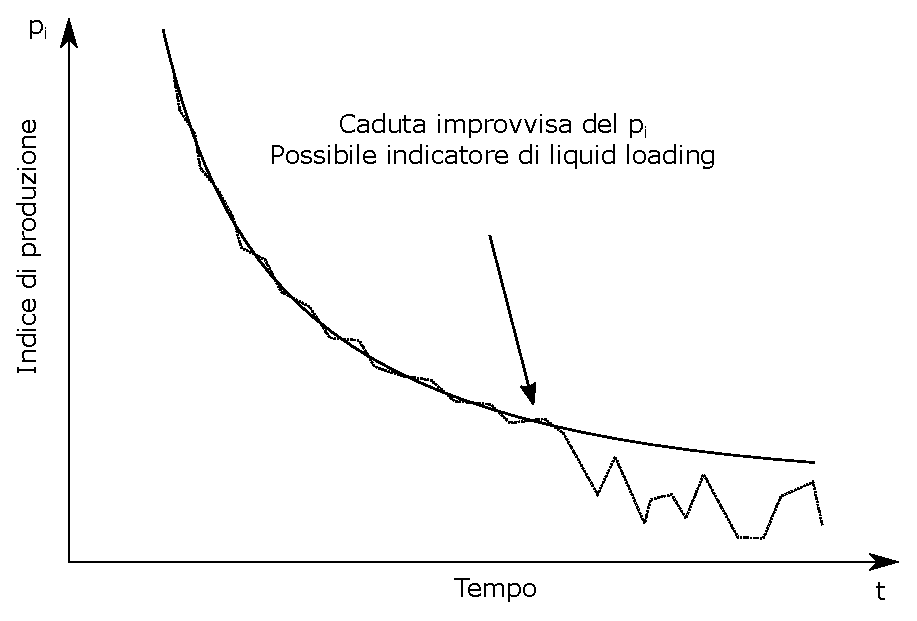
\includegraphics[width=.8\textwidth]{fig/foamer/declinecurve.eps}
    \caption{Schematizzazione del ciclo di un pozzo a gas, combinata con l'analisi della curva di declino \parencite{lea2011gas}}
    \label{fig:declinecurve}
\end{figure}

In caso di aumento del battente idrostatica, il pozzo produce gas in quantità minore rispetto alle stime effettuate. Raggiunto uno stato critico di produzione, il giacimento non ha più energia sufficiente per lo spiazzamento del pozzo e l'effetto combinato di precipitazione di liquidi a fondo pozzo e diminuzione fisiologica della pressione di giacimento porta all'innalzamento della colonna idrostatica. L'aumento dell'altezza della colonna di liquido può quindi interferire sulla produzione, sancendo così il termine del ciclo di vita del pozzo stesso.
 
\subsection{Sorgenti di liquidi per un pozzo a gas}
Nella maggior parte dei pozzi la produzione di gas è associata a produzione di liquidi. Questi liquidi possono essere acqua, vapore acqueo condensato o idrocarburi condensati. I liquidi prodotti in pozzo dipendono dalle condizioni e dal tipo di giacimento in questione. Le principali cause possono essere:

\begin{itemize}
    \item \textbf{\textit{water coning}}: fenomeno locale di deformazione del contatto gas-acqua causato dalla variazione di pressione indotta dalla produzione. Il rischio è maggiore in presenza di pressioni capillari elevate, a causa delle quali può esistere una estesa zona di frangia in cui sono mobili sia l’acqua che gas, con mobilità dell'acqua molto vicina a quella del gas;
    \item \textbf{innalzamento dell'acquifero}: in caso di acquifero attivo, il battente idrostatico raggiunge gli spari con il diminuire della pressione di giacimento;
    \item \textbf{vapore acqueo condensato}: poiché nei giacimenti è  presente acqua di strato, il gas naturale è associato a vapore acqueo. Se le condizioni di pressione e temperatura sono tali da scendere al di sotto del punto di rugiada, il vapore acqueo condensa e contribuisce al quantitativo totale di acqua di produzione;
    \item \textbf{idrocarburi condensati}: come il vapore acqueo, alcuni idrocarburi pregiati possono passare dallo stato gassoso allo stato liquido con il variare delle condizioni di pressione e temperatura;
    \item \textbf{\textit{fingering}} o \textbf{canalizzazioni}: specialmente in pozzi completati a foro scoperto o in alcuni casi di spari multipli, è possibile che dei liquidi possano confluire nel pozzo per vie preferenziali. Si verifica spesso nel caso di ammassi rocciosi particolarmente fratturati (e.g. carbonati fratturati).
\end{itemize}

\subsection{Velocità critica}
La velocità terminale è definita come la velocità di caduta di un corpo libero (particelle liquide) in un mezzo fluido (gas naturale) sotto l'influenza della forza di gravità. La velocità critica è legata alla velocità terminale delle particelle di liquido e la differenza tra le due grandezze rappresenta l'incremento utile per lo spiazzamento del liquido dal pozzo. Il primo a creare un modello sperimentale inerente al trascinamento continuo di liquido fu \textcite{turner1969analysis}. L'equazione teorica per la velocità critica \(w_t\) per il trascinamento verticale di una goccia:
\[w_t= 1,593\dfrac{\sigma{(\rho_L-\rho_G)}}{\rho_G^2}^{1/4} \qquad\textrm{[ft/sec]} \addtag \label{eq:turnerwc} \]
dove \(\sigma\) è la tensione superficiale,\(\rho_G\) e \(rho_L\) sono la densità rispettivamente del gas e del liquido.\\
Poiché in campo le condizioni variano molto rispetto al modello teorico, l'autore fornisce due equazioni relative al trascinamento di acqua (\(w_{c,W}\)) o condensati (\(w_{c,COND}\)), in funzione della pressione \(p\):
\[w_{c,W} = 5,304 \dfrac{(67-0,0031p)^{1/4}}{\sqrt{0,0031p}}  \qquad\textrm{[ft/sec]} \label{eq:w_c,w} \addtag\]
\[w_{c,COND} = 4,03 \dfrac{(45-0,0031p)^{1/4}}{\sqrt{0,0031p}}  \qquad\textrm{[ft/sec]} \label{eq:w_c,cond} \addtag\]
 Dalla \eqref{eq:w_c,w} e la \eqref{eq:w_c,cond} si ricava il valore della portata critica giornaliera:
\[Q_{c,giorno}=\dfrac{3,06 \; w_c \; p \; A}{T \; Z}  \qquad \textrm{[MMft\ap{3}/giorno]} \addtag \]
dove \(w_c\) fa riferimento o alla velocità critica per acqua o condensati. Nel caso in cui siano presenti sia acqua che condensati, per il calcolo di \(w_c\)si fa riferimento alla sola \eqref{eq:w_c,w}. Tutte i parametri e le variabili del modello sono espressi nel sistema consuetudinario statunitense. \\
Negli anni successivi la ricerca ha portato alla creazione di ulteriori modelli sempre più raffinati: \textcite{coleman1991new} utilizza il modello di \citeauthor{turner1969analysis} ma lo convalida per pressioni di testa pozzo sopra i 35 bar, \textcite{li2001new} crea un modello basato sulla forma appiattita delle particelle liquide, \textcite{nosseir1997new} formula un modello che si adatta alle condizioni di flusso.

\subsection{NODAL* analysis™}
La NODAL* analysis™ è un marchio Schlumberger ed è uno strumento analitico utile per valutare le performance di produzione di un pozzo. La NODAL* analysis™ viene impiegata per la progettazione del completamento del pozzo, considerando le caratteristiche del sistema produttivo quali afflusso, eventuali restringimenti o limiti generici. La NODAL* analysis™ si svolge tramite la definizione delle seguenti curve:
\begin{itemize}
    \item \textbf{\textit{Inflow Production Relationship} (IPR)}: curva empirica, valuta le potenzialità del reservoir tramite la portata massima o AOF (\textit{Absolute Open Flow});
    \item \textbf{\textit{Vertical Lift Performance} (VLP)}: definita la dimensione del tubino di produzione, la lunghezza (profondità) il rapporto gas-liquido, la curva esprime la pressione a fondo pozzo in funzione della portata e della pressione a testa pozzo. 
\end{itemize}
La produttività del pozzo si ottiene dall'intersezione dell'IPR con la VLP. Il punto trovato viene definito punto operativo ottimale, dove i valori di pressione e portata sono uguali in ambo le curve. Se si traccia sullo stesso grafico il valore di portata critica (\figref{fig:ipr-tpr}), si può stabilire se le condizioni operative ottimali impediscono la precipitazione della fase liquida a fondo pozzo. Se il punto di intersezione tra l'IPR e la TPR si trova a destra della curva relativa alla velocità critica, il pozzo ha energia sufficiente per trascinare interamente la fase liquida, altrimenti si incorre nel fenomeno di \textit{liquid loading}.

\begin{figure}[htbp]
    \centering
    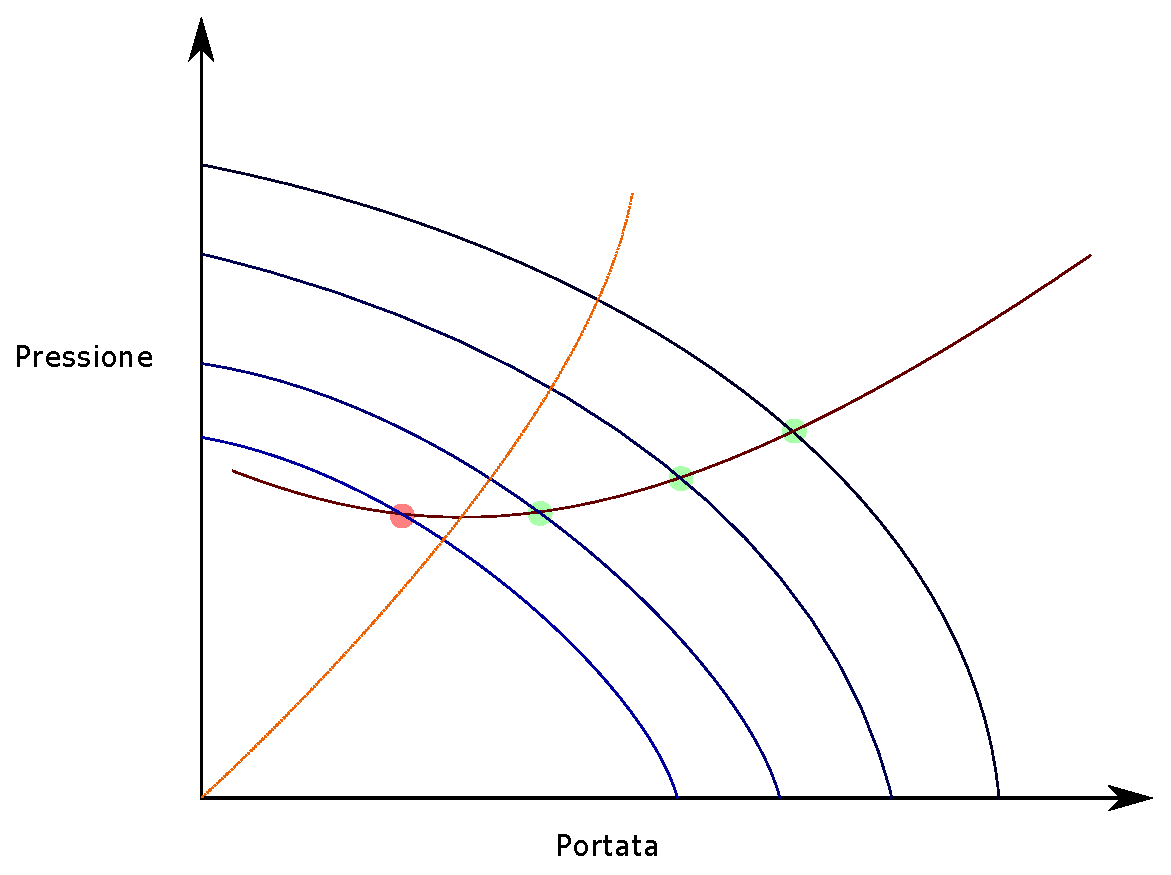
\includegraphics[width=.5\textwidth]{fig/foamer/ipr-tpr.eps}
    \caption{Schematizzazione dell'analisi nodale combinata alla portata critica di trascinamento}
    \label{fig:ipr-tpr}
\end{figure}


\section[Sollevamento artificiale per GDW]{Sistemi di sollevamento artificiale per il Gas Well Deliquification}
\sectionmark{Sollevamento artificiale per GDW}
L'industria del gas utilizza numerosi metodi per la rimozione di liquidi dai pozzi. Qui di seguito sono presentati i metodi più utilizzati e ormai consolidati nel tempo con particolare attenzione agli schiumogeni a cui è dedicata una sezione a parte. \textcite{oyewole2008artificial} classifica i sistemi di sollevamento artificiale in:
\begin{itemize}
    \item \textbf{a energia del giacimento}: qui definiti  a energia interna, i sistemi non aumentano direttamente l'energia del giacimento, bensì agiscono sui parametri che caratterizzano il trascinamento del liquido in pozzo;
    \item \textbf{a energia esterna}: sistemi a fondo pozzo che agiscono indipendentemente dall'energia residua del giacimento.
\end{itemize}
Le \textit{velocity string}, i compressori, i \textit{plunger} e gli schiumogeni sono sistemi di sollevamento artificiale a energia interna, pompe e iniezione di fluidi sono invece sistemi a energia esterna.

\subsection{Velocity string}
La \textit{velocity string} è costituita da un tubino di produzione con diametro inferiore rispetto a quello già presente in pozzo. Per produzione costante, il restringimento della sezione di produzione provoca un aumento della velocità del flusso in condotta e il superamento del valore della velocità critica. L'applicazione può avvenire su un tratto specifico del pozzo (\figref{fig:velocitystring-fixed}) oppure su tutta la sua lunghezza (\figref{fig:velocitystring-long}).

\begin{figure}[htbp]
\centering
    \subfloat[][Lunghezza fissa]
    {\makebox[0.4\textwidth]{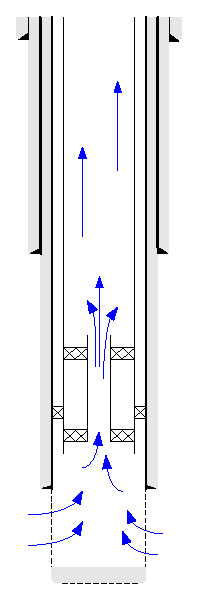
\includegraphics[width=.15\textwidth]{fig/foamer/velocitystring/velocitystring-fixed.eps}} \label{fig:velocitystring-fixed}} \quad
    \subfloat[][Su tutto il pozzo]
    {\makebox[0.4\textwidth]{\includegraphics[width=.15\textwidth]{fig/foamer/velocitystring/velocitystring-long.eps}}\label{fig:velocitystring-long}}
    \caption{Schema di applicazione della velocity string \parencite{arachman2004liquid}} 
    \label{fig:velocitystring}
\end{figure}

L'installazione della \textit{velocity string} è generalmente molto economica rispetto ad altre sistemi di sollevamento artificiale, visto che l'applicazione può avvenire anche tramite \textit{coiled tubing}, prodotti tubolari continui a sezione limitata, fabbricati in lunghezza e avvolti attorno a una bobina di raccolta \parencite{international2014introduction}. Tuttavia la progettazione deve avvenire con particolare cautela, visto che il restringimento della sezione di produzione si traduce non solo in termini di aumento di velocità, ma anche di aumento delle perdite di carico per attrito. La \textit{velocity string} non è considerata una soluzione definitiva per il GWD, dal momento che il dimensionamento ideale del tubino di produzione ausiliario cambia con l'evoluzione delle condizioni del giacimento.

\subsection{Compressione}
Possono essere impiegati dei compressori di testa pozzo per diminuire la pressione a testa pozzo. La modalità di compressione può essere a opera di un singolo compressore (\figref{fig:compressore}) o di un sistema di compressori posti in superficie. 

\begin{figure}[htbp]
    \centering
    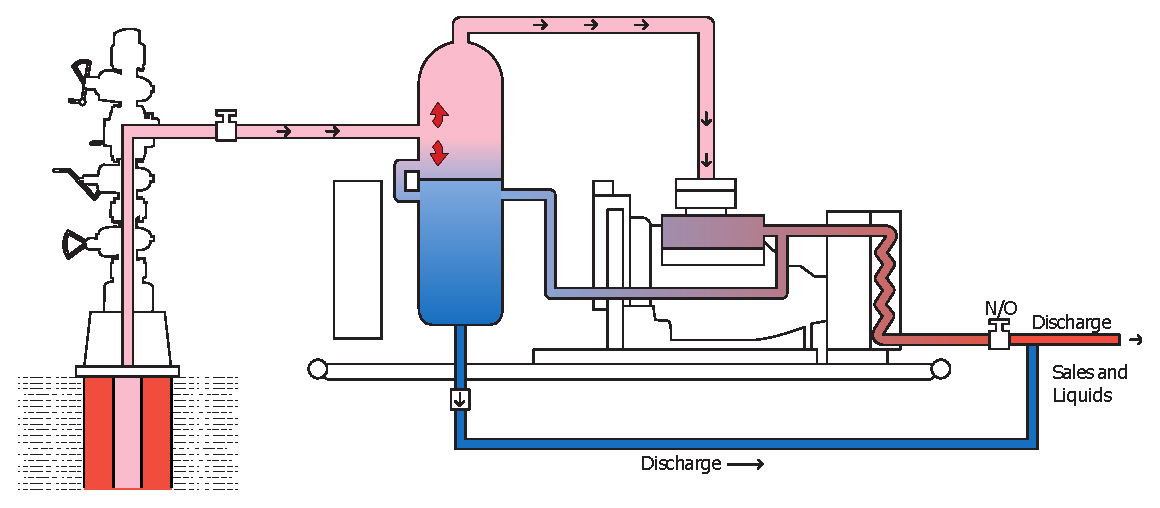
\includegraphics[width=\textwidth]{fig/foamer/compressore.eps}
    \caption{Layout semplificato del GasJack™, copressore singolo utilizzato per operazioni di compressione della testa pozzo \parencite{garner2009backside}}
    \label{fig:compressore}
\end{figure}

Una minore pressione a testa pozzo porta all'aumento dell'afflusso di gas dal giacimento. L'aumento di portata è associato all'aumento della velocità del gas, raggiungendo così valori al di sopra della velocità critica. Il dimensionamento dell'impianto di compressione si basa sulla pressione di aspirazione e la pressione di mandata, ovvero dal rapporto di compressione. \'E importante tenere presente che una minima variazione delle pressioni di aspirazione o di mandata può aumentare in maniera significativa la potenza richiesta dal compressore. La compressione e la riduzione della pressione a testa pozzo sono generalmente le prime soluzioni impiegate per il sollevamento artificiale. L'installazione dei compressori può avvenire durante il ciclo di vita del pozzo senza evidenti segnali di \textit{liquid loading}: la diminuzione di pressione consente di lavorare in condizioni migliori, aumentando le performance generali e quindi la produzione di gas giornaliera. La compressione può anche considerarsi un sistema di sollevamento artificiale ausiliario: un compressore può interfacciarsi con altre soluzioni come agenti surfattanti, \textit{gas lift}, \textit{plunger}, \textit{beam pump}, ESP o \textit{velocity string}, aumentando in modo significativo le performance di \textit{liquid unloading}. 

\subsection{Plunger}
I plunger sono dei dispositivi installati all'interno del pozzo per la rimozione meccanica di liquidi e altri agenti contaminanti. Il \textit{plunger} è un pistone tuffante che viaggia liberamente dal fondo pozzo alla superficie, spinto da una pressione che deve essere sufficiente a trascinare sia il dispositivo che i fluidi accumulati. La produzione di gas con l'installazione di un \textit{plunger} risulta discontinua, legata alla ciclicità dello strumento che deve percorre in entrambe le direzioni tutta la lunghezza del pozzo. Come si può vedere nella \figref{fig:conventionalplunger} l'applicazione di un \textit{plunger} in pozzo richiede determinata strumentazione di superficie (valvole) e di fondo pozzo (\textit{plunger} e meccanismo a molla). Una tipica installazione convenzionale è organizzata nel seguente modo:

\begin{itemize}
    \item \textbf{\textit{bumper} a molla}, utile a ricevere il \textit{plunger} a fondo pozzo e evitare danni dovuti all'impatto a terra;
    \item \textbf{ricevitore di superficie}, blocca il \textit{plunger} una volta giunto in superficie e consente il deflusso del gas in condotta;
    \item \textbf{valvola motorizzata di superficie}, controllata elettronicamente, apre e chiude il pozzo quando necessario;
    \item \textbf{sensore elettronico di superficie}, si attiva quando il \textit{plunger} giunge in superficie;
    \item \textbf{controller elettronici}, con ciclicità impostata da operatore, gestisce tutte le operazioni di produzione e registra dati in continuo.
\end{itemize}

\begin{figure}[htbp]
    \centering
    \includegraphics[width=0.6\textwidth]{fig/foamer/plunger-installation.eps}
    \caption{Tipica installazione di \textit{plunger} \parencite{lea2011gas}}
    \label{fig:plunger-installation}
\end{figure}

Come già detto, l'applicazione di un plunger convenzionale trasforma la produzione da continua a ciclica, caratterizzata quindi da \textit{shut-in} programmati per far tornare il \textit{plunger} alla posizione originaria e permettere al pozzo, in caso di bisogno, di raggiungere una pressione tale da poter trascinare il \textit{plunger} assieme alla colonna di fluido presente. La \figref{fig:conventionalplunger} mostra un generico ciclo di produzione convenzionale:
\begin{enumerate}
    \item[(a)] \textit{plunger} a fondo pozzo con liquido al di sopra, valvola di superficie chiusa;
    \item[(b)] apertura della valvola di superficie e risalita del \textit{plunger} assieme alla colonna liquida;
    \item[(c)] fase produttiva del pozzo in assenza di cadute di pressione dovute a \textit{liquid loading};
    \item[(d)] riaccumulo di fluido a fondo pozzo;
    \item[(e)] chiusura del pozzo e discesa del \textit{plunger} a fondo pozzo.
\end{enumerate}

\begin{figure}[htbp]
    \centering
    \subfloat[][]
    {\centering \includegraphics[height=.3\textheight]{fig/foamer/plunger-conventional/conventionalplunger-A.eps}} \label{fig:plunger-conventional-A} \qquad \qquad
    \subfloat[][]
    {\centering \includegraphics[height=.3\textheight]{fig/foamer/plunger-conventional/conventionalplunger-B.eps} \label{fig:plunger-conventional-B}}  \qquad \qquad
    \subfloat[][]
    {\centering \includegraphics[height=.3\textheight]{fig/foamer/plunger-conventional/conventionalplunger-C.eps} \label{fig:plunger-conventional-C}} \qquad \qquad
    \subfloat[][]
    {\centering \includegraphics[height=.3\textheight]{fig/foamer/plunger-conventional/conventionalplunger-D.eps} \label{fig:plunger-conventional-D}} \qquad \qquad
    \subfloat[][]
    {\centering \includegraphics[height=.3\textheight]{fig/foamer/plunger-conventional/conventionalplunger-E.eps} \label{fig:plunger-conventional-E} }
    \caption{Ciclo di un plunger convenzionale}
    \label{fig:conventionalplunger}
\end{figure}

In commercio esistono varie tipologie di \textit{plunger} e variano a seconda della geometria e degli inserti installati sulla superficie esterna (e.g. spazzole per la pulizia del tubino di produzione). Negli ultimi anni sono nati nuovi sistemi definiti a ciclo libero o in continuo, che permettono la discesa senza interrompere la produzione. Numerosi sono i brevetti e i prodotti che offrono \textit{plunger-lift} in continuo: possono essere dotati di una valvola interna (e.g. Weatherford RapidFlo™, FB FreeCycle™ o McClain™) oppure a due pezzi (e.g. Peacemaker™, composto da una sfera e un manicotto). La \figref{fig:plunger} mostra alcune tipologie presenti sul mercato.\\
L'applicazione di \textit{plunger} in pozzo per il sollevamento artificiale richiede un investimento iniziale relativamente basso, ma dei costi operativi che possono incidere col tempo e portare a un aumento imprevisto del costo di produzione del gas. Gli investimenti iniziali indiretti possono però incidere fortemente sulla scelta del \textit{plunger}: la variazione dei volumi di gas e liquido rende necessaria una nuova valutazione circa il dimensionamento degli impianti di trattamento a valle del pozzo, i costi iniziali possono essere quindi legati per esempio all'installazione di un nuovo separatore.

\begin{figure}[htbp]
\centering
    \subfloat[][A spirale]
    {\makebox[0.2\textwidth]{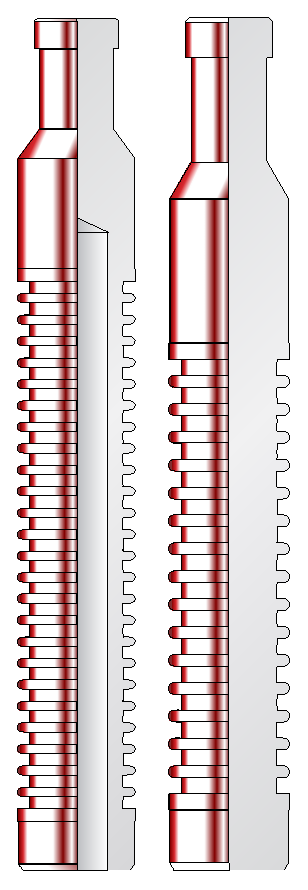
\includegraphics[height=.25\textheight]{fig/foamer/plunger/plunger-spiral.eps}} \label{fig:plunger-spiral}} \quad
    \subfloat[][T-pad]
    {\makebox[0.2\textwidth]{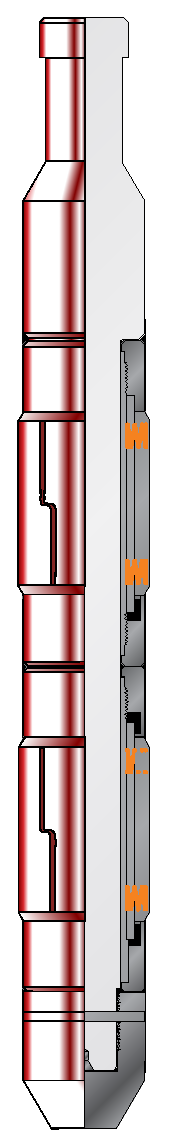
\includegraphics[height=.25\textheight]{fig/foamer/plunger/plunger-tpad.eps}} \label{fig:plunger-tpad}}  \quad
    \subfloat[][A spazzole fisse]
    {\makebox[0.2\textwidth]{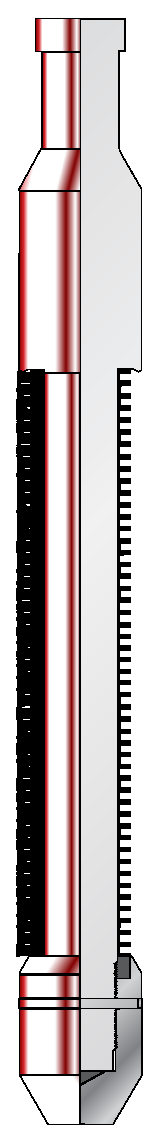
\includegraphics[height=.25\textheight]{fig/foamer/plunger/plunger-fixedbrush.eps}} \label{fig:plunger-fixedbrush}} \quad
    \subfloat[][RapidFlo™]
    {\makebox[0.25\textwidth]{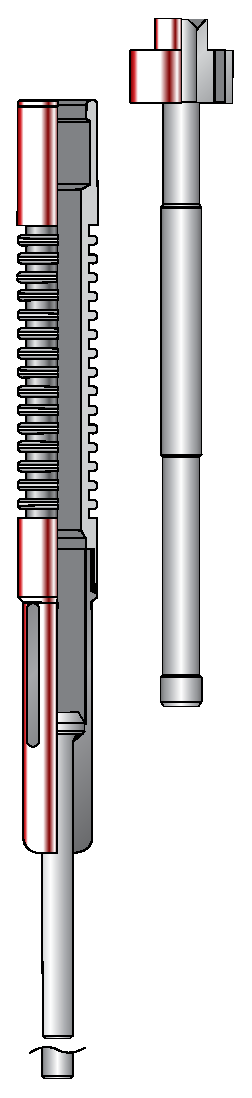
\includegraphics[height=.25\textheight]{fig/foamer/plunger/plunger-rapidflo.eps}} \label{fig:plunger-rapidflo} }
\caption{Principali tipologie di \textit{plunger} proposte da Weatherford \parencite{weatherford2008brochure}}
\label{fig:plunger}
\end{figure}

\subsection{Altri sistemi di sollevamento artificiale per deliquification} \subsectionmark{Altri sistemi per GWD}
Alcune tecnologie per l'attenuazione del battente idrostatico in pozzo nascono da applicazioni pensate in origine per il sollevamento artificiale di giacimenti a olio. Questi sistemi sono stati riadattati per il trascinamento dell'acqua a fondo pozzo o per agevolare l'afflusso del gas in pozzo. I sistemi presentati nel paragrafo corrente sono tutti a energia esterna.
\paragraph{Gas lift}
Il \textit{gas lift} per \textit{deliquification} consiste nell'iniezione di gas da una fonte esterna al pozzo a una certa profondità. Nel campo dell'olio il gas iniettato a fondo pozzo diminuisce il peso della colonna, facilitando così il flusso in condotta. Nel caso dei pozzi a gas viene fatto fluire gas a fondo pozzo sia per diminuire la densità della colonna idrostatica, sia per aumentare la produzione di gas effettiva, quindi l'efficacia di trascinamento della colonna da parte della corrente gassosa. Questo sistema gode il vantaggio di non provocare significative variazioni delle condizioni di produttività e riesce a lavorare anche in pozzi deviate. L'applicazione purtroppo dipende fortemente dalla presenza di una sorgente di gas ad alta pressione, rappresentata da un pozzo nella zona limitrofe o a cui però sono associati dei costi operativi.
\paragraph{Sistemi di pompaggio}
Le pompe a cavalletto (\textit{Beam Pump}, BP), impiegate in modo massiccio per il sollevamento artificiale per giacimenti a olio, rappresentano il sistema di pompaggio più comune anche nel GWD. Generalmente i sistemi di pompaggio spingono la colonna idrostatica lungo il tubino di produzione (o un tubino ausiliario, come un \textit{coiled tubing} installato a posteriori) e il gas prodotto viene fatto fluire nell'annulus. Altri sistemi di pompe utilizzate anche in questo campo sono le pompe elettriche sommerse (\textit{Electrical Submersible Pump},   ESP), pompe a cavità progressiva (\textit{Progressing Cavity Pump}, PCP) e pompe idrauliche (a pistone o \textit{jet pump}). Le pompe vengono generalmente impiegate quando la pressione a fondo pozzo è relativamente bassa e quando il rapporto gas/liquido non è sufficiente da garantire lo spiazzamento della colonna idrostatica tramite i sistemi a energia interna. Le pompe non possono operare in presenza di gas, perciò vanno opportunamente collocate al di sotto degli spari, in modo da ottenere una buona separazione del liquido dal gas. La vita media delle pompe dipende fortemente dagli agenti di erosione, è importante capire se la produzione di liquidi e gas comporta anche la produzione di sabbia.

\section{Schiumogeni}
L'impiego di schiumogeni nell'industria petrolifera è vario e ormai consolidato nel tempo. Come visibile in \tabref{tab:surfactantapplications} i tensioattivi sono impiegati in tutte le fasi di recupero del greggio e nell'industria di processo, dalle perforazioni, iniezioni in giacimento, produzione, al trasporto in condotta onshore e offshore.

\begin{table}[htbp]
    \small
    \centering
    \caption{Alcuni esempi di applicazioni di tensioattivi nell'industria petrolifera; e fasi G, W e O rappresentano rispettivamente il gas, l'acqua e l'olio \parencite{schramm2006emulsions}.}
    \label{tab:surfactantapplications}
\begin{tabular}{p{.8\textwidth}p{.1\textwidth}}
\hline
{\bf Applicazione}                                                         & {\textbf{Fasi}}           \\ \hline
Fluidi di perforazione con schiume                                         & G/W                    \\
Fluidi di stimolazione e fratturazione con schiume                         & G/W                    \\
Fluidi acidificanti con schiume                                            & G/W                    \\
Recupero di olio freddo e pesante tramite schiume                          & G/O                    \\
Schiume di processo della flottazione dell'olio                            & G/O                    \\
Schiume antincendio                                                        & G/W                    \\
Emulsioni per olio pesante in condotta                                     & O/W                    \\
Emulsioni per la stimolazione pozzo                                        & O/W                    \\
Flottazione di miscele a olio e sabbie bituminose                          & O/W                    \\
Fluidi di perforazione emulsionati (fanghi a base olio)                    & W/O                    \\
Emulsione di catrame e bitumi                                              & O/W                    \\
Emulsioni in situ per EOR                                                  & O/W                    \\
Emulsione di carburanti di trasporto (70\% olio pesante)                   & O/W                    \\
Schiume per il controllo della mobilità del gas                            & G/W                    \\
Sospensioni per fluidi (fanghi) di perforazione                            & S/W                    \\
Sospensioni per fratturazione idraulica e stimolazione del pozzo           & S/W                    \\
Impasti cementizi in pozzo                                                 & S/W                    \\
Solidi di produzione a testa pozzo nel recupero primario dell'olio pesante & S/W                    \\ \hline
\end{tabular}
\end{table}

I tensioattivi sono utilizzati anche in pozzo per mitigare i fenomeni di \textit{liquid loading} e la tecnica ha ormai acquisito notevole importanza nel GWD. I tensioattivi sono introdotti in pozzo in tre modi:
\begin{itemize}
    \item \textit{\textbf{schiumogeni in stick}}: barre solide di sapone introdotte lungo il tubino di produzione senza la necessità di interrompere la produzione;
    \item \textbf{schiumogeni liquidi in-batch}: viene chiuso il pozzo e viene immesso lungo il tubino di produzione un certo volume di surfactanti seguiti da una soluzione salina, per poi riaprire il pozzo dopo aver atteso la discesa del surfactante;
    \item \textbf{schiumogeni liquidi in continuo}: una \textit{capillary string}, collegata a una pompa dosatrice, viene calata lungo il pozzo fino all'altezza degli spari, lo schiumogeno liquido viene iniettato durante la produzione di gas.
\end{itemize}
 Gli \textit{stick} sono facili da utilizzare, non comportano modifiche di impianto e rappresentano il metodo più economico. Tuttavia interessano solo la parte superiore della colonna liquida e rimuovono parzialmente l'acqua a fondo pozzo; inoltre, essendo solubili in acqua, non agiscono in modo appropriato in presenza di idrocarburi condensati sull'interfaccia gas-liquido \parencite{bolding2007resurrecting}. Gli schiumogeni liquidi o anche detti \textit{foamer}, pur avendo costi maggiori e richiedendo maggiori accorgimenti per il loro utilizzo, sono molto più performanti, hanno la capacità di interessare tutta la colonna idrostatica e non sono influenzati dalla presenza di idrocarburi condensati (gli schiumogeni in-batch sono spinti da un \textit{chaser}, gli schiumogeni in continuo agiscono alla base del pozzo). Nel seguente paragrafo si farà riferimento ai soli \textit{foamer}, descrivendo i principi e le procedure operative per il sollevamento artificiale tramite tensioattivi liquidi.
 
\subsection{Tensioattivi}
I tensioattivi, surfactanti o agenti attivi di superficie sono composti organici composti al massimo da un gruppo, testa, liofilo e un gruppo, coda, liofobico \figref{fig:sls}. Si parla di testa idrofila e coda idrofoba se il solvente nel quale deve essere utilizzato il tensioattivo è acqua o a base acqua. In termini chimico-fisici la struttura di un surfactante è costituita da un gruppo polare e da un gruppo apolare . La \figref{fig:sls} mostra un esempio di struttura chimica di un tensioattivo con in evidenza il gruppo polare e apolare.

\begin{figure}[htbp]
    \centering
    \includegraphics[width=.8\textwidth]{fig/foamer/sls.eps}
    \caption{Laurilsolfato di sodio, tensioattivo anionico utilizzato in molte famiglie di prodotti domestici. La catena a 12 atomi di carbonio rappresenta il gruppo apolare (in blu) mentre il gruppo solfato associato allo ione sodio rappresenta il gruppo polare (in viola).}
    \label{fig:sls}
\end{figure}

I surfactanti sono classificati in base alla carica del gruppo polare (\figref{fig:surfactants-classification}):
\begin{itemize}
    \item \textbf{anionici}: in genere sali costituiti da lunghe catene con atomi di carbonio che terminano con un gruppo carbossilato, solfonato o fosfato;
    \item \textbf{cationici}: sali di cui è importante la parte positiva, costituita da lunghe catene di atomi di carbonio terminanti con un gruppo ammonico;
    \item \textbf{non ionici}: alcoli a lunga catena, come i derivati poliossietilenici degli acidi grassi;
    \item \textbf{anfoteri} o \textbf{zwitterionici}: tensioattivi anionici in ambiente alcalino, tensiattivi cationici in ambiente acido.
\end{itemize}

\begin{figure}[htbp]
    \centering
    \subfloat[][Anionici]
    {\includegraphics[width=.45\textwidth]{fig/foamer/surfactants-classification/anionic.eps} \label{fig:anionic}} \quad
    \subfloat[][Cationici]
    {\includegraphics[width=.45\textwidth]{fig/foamer/surfactants-classification/cationic.eps} \label{fig:cationic}}  \\
    \subfloat[][Anfoterici]
    {\includegraphics[width=.45\textwidth]{fig/foamer/surfactants-classification/anphoteric.eps} \label{fig:anphoteric}}  \quad
    \subfloat[][Non ionici]
    {\includegraphics[width=.45\textwidth]{fig/foamer/surfactants-classification/nonionic.eps} \label{fig:nonionic}} 
\caption{Classificazione dei tensioattivi in base alla carica del gruppo polare.}
\label{fig:surfactants-classification}
\end{figure}

Si consideri un volume d'acqua a contatto con aria dove vengono disciolti dei tensioattivi. I surfactanti, in prossimità della superficie di contatto delle due fasi, si orientano in modo tale che il gruppo polare sia adsorbito dalla fase liquida e il gruppo apolare permanga nella fase gassosa. Tale adsorbimento porta alla diminuzione dell'energia libera di Gibbs o entalpia libera, quindi alla riduzione della tensione superficiali tra le due fasi. Allo stesso modo i tensioattivi possono diminuire la tensione superficiale dell'acqua a contatto con una generica fase olio o di un solido, aumentando la bagnabilità di quest'ultimo.

Un altro modo per limitare il contatto del gruppo apolare con l'acqua è la creazione di strutture bi- o tridimensionali, capaci di racchiudere i gruppi apolari internamente e mettendo a contatto con l'acqua i gruppi polari (\figref{fig:micelle}). Queste strutture sono definite micelle, sono il frutto dei fenomeni di aggregazione dei tensioattivi e possono avere forma lamellare (in questo caso i surfactanti sono molecole anfifiliche o anfifobiche), sferica o cilindrica.  Tali aggregati supramolecolari tendono a crearsi una volta superato una certa concentrazione del surfactante in soluzione, definita concentrazione micellare critica (CMC). La complessità di tali strutture dipende dalla concentrazione in acqua e dalla specie chimica dell'agente attivo di superficie.

\begin{figure}[htbp]
    \centering
    \includegraphics[width=.5\textwidth]{fig/foamer/micelle.eps}
    \caption{Sezione parziale di una micella anionica, il layer compatto negativo generato dall'orientamento del gruppo polare del tensioattivo è circondato dalla fase acqua  \parencite{attwood2012fasttrack}.}
    \label{fig:micelle}
\end{figure}

\subsection{Schiuma}
Viene definita schiuma una dispersione stabile di gas in un liquido. Se si introduce un flusso di aria all'interno di un liquido, le bolle così prodotte assumono una forma sferica. Poiché l'aria ha densità minore dell'acqua queste tenderanno a salire in superficie. Se il liquido in questione è privo di surfactanti in soluzione, le bolle non sono stabili e si dissolvono spontaneamente (\figref{fig:foam-stability-nonsurfactants}). Non è possibile quindi creare una schiuma stabile in un liquido senza la presenza di surfactanti. In liquidi con tensioattivi in soluzione, le bolle sono rese stabili grazie all'azione degli agenti attivi di superficie, che creano un film attorno alle bolle di gas. Una volta giunte in superficie, le bolle presentano un doppio strato o doppio film di tensioattivi sulla superficie (\figref{fig:foam-stability-surfactants}).

\begin{figure}[htbp]
    \centering
    \subfloat[][Liquidi senza tensioattivi]
    {\includegraphics[height=.222\textheight]{fig/foamer/foam-stability/non-surfactants.eps} \label{fig:foam-stability-nonsurfactants}} \quad
    \subfloat[][Liquidi con tensioattivi]
    {\includegraphics[height=.222\textheight]{fig/foamer/foam-stability/surfactants.eps} \label{fig:foam-stability-surfactants}}
    \caption{Insufflazioni nel liquido e generazione delle bolle d'aria \parencite{tego2014brochure}.}
    \label{fig:surfactants-stability}
\end{figure}

Le bolle appena generate all'interno del liquidi, dalle piccole dimensioni e pressoché identiche, sono definite microbolle; le bolle visibili sulla superficie sono definite macrobolle. In un primo momento la schiuma generata è ricca in liquidi, le bolle hanno configurazione sferica e sono stabili grazie a spesse lamelle liquide a doppio strato di tensioattivo. Con il tempo la forza di gravità agisce sulla fase liquida della schiuma, che defluisce così verso il basso: il processo è definito drenaggio per gravità \parencite{tego2014brochure}. Si distinguono quindi due configurazioni di schiuma, prima e dopo il processo di drenaggio (\figref{fig:lamella}):
\begin{itemize}
    \item \textbf{schiuma bagnata}: bolle sferiche e contributo importante della fase liquida;
    \item \textbf{schiuma asciutta}: struttura poliedrica dettata dalla bassa presenza di liquido e caratterizzata da lamelle di schiuma molto elastiche.
\end{itemize}

\begin{figure}[htbp]
    \centering
    \includegraphics[width=.6\textwidth]{fig/foamer/lamella.eps}
    \caption{Struttura della schiuma e stabilizzazione della lamella a opera dei surfactanti \parencite{tego2014brochure}.}
    \label{fig:lamella}
\end{figure}

Il processo di drenaggio non è però sufficiente ad abbattere la schiuma. Si raggiunge un punto in cui il drenaggio non è più possibile poiché le alte concentrazioni di tensioattivi sono tali che le forze di repulsione elettrostatica e sterica impediscono un'ulteriore contrazione delle lamelle. La schiuma è quindi definita stabile quando si instaura uno stato di equilibrio tra il drenaggio per gravità e le forze di repulsione tra molecole.
Le sottili lamelle di schiuma, oltre ad essere stabili, sono molto elastiche. Un aumento della superficie delle lamella, provocato dalla deformazione della bolla, porta alla riduzione locale della concentrazione di surfactanti e di conseguenza a un aumento locale della tensione superficiale della lamella stessa. L'elasticità di Gibbs-Marangoni consente quindi alla schiuma, se sollecitata dall'esterno, di tornare alla configurazione geometrica iniziale.

\subsection{Antischiuma}
Gli antischiuma o \textit{defoamer} sono agenti chimici capaci di penetrare la struttura lamellare della schiuma, destabilizzando la struttura della bolla per farla così esplodere. Le caratteristiche principali di un buon antischiuma sono:
\begin{itemize}
    \item insolubilità nella soluzione generatrice di schiuma;
    \item bassa tensione superficiale;
    \item coefficiente di penetrazione (\(E\)) positivo;
    \item coefficiente di espansione (\(S\)) o coefficiente di \textit{bridging} positivo oppure caratteristiche di \textit{dewetting}.
\end{itemize}

L'insolubilità del \textit{defoamer} non deve essere assoluta: l'antischiuma deve pur sempre essere sufficientemente compatibile con il mezzo da trattare. 
Come già detto il \textit{defoamer} deve penetrare la lamella in modo da disgregare le bolle della schiuma. Un prerequisito fondamentale è quindi la capacita di penetrare il film di tensioattivi. La capacità penetrante dell'antischiuma è espressa fisicamente dal coefficiente di penetrazione \(E\):
\[E = \sigma_{L/G} + \sigma_{L/D} + \sigma_{D/G} \label{eq:penetration} \]
dove \(\sigma\) rappresenta la tensione superficiale e fa riferimento alla fase liquido-gas (\(L/G\)), liquido-defoamer (\(L/D\)) e \textit{defoamer}-gas (\(D/G\)). Solo se \(E\) è positivo, l'antischiuma è capace di permanere sulla parete della lamella, altrimenti rimane all'interno della soluzione liquida. Giunta sul film di surfactanti,  la gocciolina di \textit{defoamer} può espandersi su tutta la superficie della lamella, formando così delle lenti. Il risultato è una diminuzione della stabilità e flessibilità della lamella che porta così alla disgregazione della bolla. Il processo di espansione porta allo scorrimento del fluido nella lamella lungo le direzioni di espansione del \textit{defoamer}. Il fenomeno è conosciuto come flusso di Marangoni e provoca un restringimento dello strato della lamella, destabilizzando ulteriormente la struttura della bolla. Il coefficiente di espansione \(S\) esprime le capacità espandenti dell'antischiuma:
\[S = \sigma_{L/G} - \sigma_{L/D} - \sigma_{D/G} \label{eq:spreading} \]

\begin{figure}[htbp]
    \centering
    \includegraphics[height=.11\textheight]{fig/foamer/penetration.png}
    \caption{Penetrazione e espansione del \textit{defoamer} sul film di tensioattivi \parencite{tego2014brochure}.}
    \label{fig:penetration}
\end{figure}

I \textit{defoamer} con insufficienti capacità espandenti possono trattare la schiuma tramite il processo di \textit{bridging}. Requisito fondamentale è la capacità dell'antischiuma di penetrare sia il film esterno della lamella, quindi un coefficiente di penetrazione positivo, sia il film interno. 

\begin{figure}[htbp]
    \centering
    \includegraphics[height=.11\textheight]{fig/foamer/bridging.png}
    \caption{Processo di bridging del \textit{defoamer} sul film di tensioattivi \parencite{tego2014brochure}.}
    \label{fig:bridging}
\end{figure}

Ciò è possibile se la lamella è sufficientemente ristretta grazie al drenaggio per gravità oppure se le bolle sono sufficientemente grandi per via del fenomeno di coalescenza. Raggiunta l'altra parete della lamella, la rottura della lamella può avvenire per allungamento o \textit{dewetting}. I due meccanismi sono possibili se il coefficiente di \textit{bridging} \(B\) è positivo:
\[B = (\sigma_{L/G})^2 + (\sigma_{L/D})^2 - (\sigma_{D/G})^2 \label{eq:bridging} \]

Se l'antischiuma agisce tramite \textit{dewetting}, la soluzione liquida non riesce a entrare totalmente in contatto con le goccioline di \textit{defoamer}. Di conseguenza, il fenomeno di \textit{dewetting} porta al collasso delle bolle generate dai tensioattivi. Anche gli agenti solidi portano al fenomeno di \textit{dewetting}.
Se il processo di rimozione di schiuma avviene tramite l'allungamento delle lamelle, le goccioline di antischiuma agiscono sul punto più debole della lamella per portarla alla lacerazione e quindi alla destabilizzazione della configurazione totale della schiuma.

\begin{figure}[htbp]
    \centering
    \includegraphics[height=.11\textheight]{fig/foamer/dewetting.png}
    \caption{Processo di dewetting del \textit{defoamer} sul film di tensioattivi \parencite{tego2014brochure}.}
    \label{fig:dewetting}
\end{figure}

Attualmente le classi di \textit{defoamer} in commercio sono:
\begin{itemize}
    \item \textbf{siliconici}: i polisilossani e suoi affini (e.g. polidimetilsilossani) appartengono al gruppo di antischiuma più comunemente utilizzati, sono polimeri costruiti su un gruppo silossano, dove al centro della molecola si alternano atomi di silicio e ossigeno, hanno grandi capacità di espansione e efficacia a largo spettro;
    \item \textbf{oli minerali}: generalmente idrocarburi alifatici e non aromatici per motivi ambientali, queste molecole apolari hanno buone capacità di espansione, hanno problemi in ambienti molto alcalini e ad alte temperature;
    \item \textbf{a base di olio vegetale}: o anche definiti antischiuma VOC-free, presentano proprietà molto simili agli oli minerali con il vantaggio di utilizzare una risorsa rinnovabile, solitamente con l'aggiunta di siliconi e cere sintetiche;
    \item \textbf{a base di polimeri}: possono essere acidi grassi modificati, polieteri o ammine modificate, la polarità di queste molecole può essere cambiata lavorando la struttura chimica e, grazie alla loro grande compatibilità, sono impiegati laddove non è possibile impiegare altri \textit{defoamer}.
\end{itemize}

\section[Applicazione di schiumogeni per GWD]{Applicazioni di schiumogeni per il Gas Well Deliquification} \label{section:foamer-ll}
L'applicazione di surfactanti o schiumogeni in pozzi caratterizzati da un battente idrostatico a fondo pozzo permette il trascinamento dei liquidi per valori di portata inferiori a quella critica e evita il riaccumulo di questi una volta spiazzato il pozzo. Si consideri la \eqref{eq:turnerwc}: \textcite{turner1969analysis} fornisce il valore della velocità critica in funzione della densità dei fluidi e della tensione superficiale fra le due fasi. L'impiego di surfactanti permette di ridurre la tensione superficiale tra i liquidi e l'acqua, così come la densità dell'acqua, trasformata in parte in schiuma. \textcite{campbell2001corrosion} definisce in via teorica che la tensione superficiale possa essere ridotta da 60 dyne/cm a 30 dyne/cm e che la densità della schiuma possa attestarsi al 20\% della densità originaria della fase liquida (\figref{fig:campbell}). Da questi valori si può facilmente calcolare che i tensioattivi permettono di ridurre la portata critica di un pozzo di circa il 30\%. \textcite{wittfeld2015foam} conferma questi dati sperimentalmente e propone una riduzione del valore di portata critica del 33\%, con picchi del 45\% su breve periodo.

\begin{figure}[htbp]
    \centering
    \includegraphics[width=\textwidth]{fig/foamer/campbell.eps}
    \caption{Tensione superficiale e densità della schiuma in funzione della concentrazione in acqua per tensioattivi attualmente disponibili sul mercato \parencite{campbell2001corrosion}.}
    \label{fig:campbell}
\end{figure}

\subsection{Schiumogeni in-batch}
L'applicazione di schiumogeni in-batch consiste nel pompaggio di un prefissato volume di tensioattivo (nell'ordine di centinaia di litri) all'interno del pozzo a intervalli prefissati. Un tipico ciclo in-batch di schiumogeno tramite sistema di pompaggio del tensioattivo (fisso o mobile) consiste in:
\begin{itemize}
    \item chiusura del pozzo;
    \item apertura valvola di isolamento superiore e aggancio manicotto sul cappelletto flangiato della croce di produzione;
    \item pompaggio del \textit{foamer};
    \item pompaggio della soluzione salina (definito in questo caso \textit{chaser});
    \item chiusura della valvola di isolamento superiore;
    \item installazione sistema di iniezione antischiuma in linea di produzione
    \item riapertura pozzo il giorno seguente.
\end{itemize}
L'esperienza in campo suggerisce l'introduzione di \textit{foamer} in pozzo in concentrazioni pari a 10000 ppm della colonna idrostatica che si desidera rimuovere. \'E difficile calcolare esattamente il volume di acqua in pozzo, è consuetudine quindi procedere con 50 litri di schiumogeno. Se l'applicazione ha successo, si tenta di diminuire il quantitativo al fine di non incorrere in fenomeni di emulsioni o inutile sovradosaggio del prodotto. Se si ipotizzano dei grossi volumi di acqua in pozzo, si consiglia un quantitativo di \textit{foamer} attorno ai 100÷150 litri.\\
Il \textit{chaser} è una soluzione salina con densità superiore di quella dell'acqua. La soluzione \textit{chaser}-schiumogeno può così spingersi in modo appropriato lungo il pozzo e, grazie alla sua densità, può così raggiungere le parti più basse della colonna liquida. Inoltre il \textit{chaser} evita l'evaporazione del \textit{foamer} in profondità, con condizioni di temperatura e pressione maggiori. Ad oggi vengono utilizzate soluzioni a base di cloruro di potassio (densità relativa \(\rho_{r,KCl}=1,05\)), fino a qualche tempo fa erano preferite soluzioni a base di cloruro di sodio (\(\rho_{r,NaCl}=1,15\)), di densità maggiore ma non più impiegate a causa della generazione spontanea di ponti salini in pozzo.\\
L'applicazione di \textit{defoamer} è fondamentale per garantire la sicurezza e il corretto funzionamento dell'impianto di trattamento del gas, la quantità di defoamer da iniettare è legata alle caratteristiche qualitative e quantitative del \textit{foamer} impiegato per lo spiazzamento dei liquidi.\\
I risultati ottenuti grazie all'impiego di schiumogeno non possono essere confermati dopo una sola prima applicazione, bensì devono essere svolti almeno 5 cicli in-batch prima di confermare l'efficacia del metodo per il pozzo in esame. Idealmente si possono verificare i benefici del \textit{foamer} solo dopo settimane di applicazioni, i pozzi a produzione discreta programmata sono quindi i più idonei per l'applicazione in batch in pozzo. La \figref{fig:bacth-cycle} mostra un pozzo con produzione intermittente regolare trattato con applicazioni di \textit{foamer} in-batch.

\begin{figure}[htbp]
    \centering
    \includegraphics[width=\textwidth]{fig/foamer/batch-cycle.eps}
    \caption{Applicazione di \textit{foamer} in-batch su un pozzo con produzione a shut-in programmati \parencite{wittfeld2015foam}.}
    \label{fig:bacth-cycle}
\end{figure}

In rosso sono indicati i batch di schiuma applicati in pozzo. L'applicazione è stata poi fermata per 6-7 settimane per verificare l'efficacia dell'impiego di tensioattivi per il sollevamento artificiale dell'acqua. L'applicazione permette di avere produzioni molto più costanti, infatti i valori di portata tra uno \textit{shut-in} e l'altro sono pressoché identici. \textcite{wittfeld2015foam} ha confermato l'efficacia dell'applicazione trattando circa 60 pozzi. Trascurando i pozzi in cui non è stato possibile applicare il \textit{foamer}, nel 50\% dei casi si sono avuti degli evidenti miglioramenti di performance, il 30\% non presenta elementi sufficienti per affermare o negare l'utilità del metodo, nel 20\% la produzione di gas non risente affatto dell'applicazione.\\
L'impiego di schiumogeni in-batch richiede condizioni specifiche per garantire una buona riuscita dell'applicazione:
\begin{itemize}
    \item \textbf{rapporto acqua-condensati (\textit{Water to Condensate Ratio}, WCR)}: gli idrocarburi condensati agiscono come antischiuma naturali e diminuiscono le performance dello schiumogeno;
    \item \textbf{tipi di condensato}: condensati di idrocarburi pesanti diminuiscono le performance della schiuma in maniera più decisa rispetto a condensati di idrocarburi leggeri;
    \item \textbf{impiego di altri prodotti chimici}: alcuni additivi chimici, come per esempio degli agenti anticorrosivi, sono conosciuti propriamente anche come \textit{defoamer};
    \item \textbf{solidi in sospensione o disciolti}: la formazione di schiuma risente della presenza di solidi nella soluzione liquida, sia sospesi (e.g. \ce{Fe S}) che disciolti (e.g. sali).
\end{itemize}

I costi di tale applicazione si aggirano a €xxx per batch e variano a seconda di quanti pozzi possono essere raggiunti in giornata: si tende quindi a trattare più pozzi nella stessa giornata al fine di spalmare i costi fissi della manodopera e della strumentazione in affitto.

\subsection{Schiumogeni in continuo}
L'applicazione di schiumogeno in continuo avviene tramite l'installazione di una \textit{capillary string} attraverso la croce di produzione, all'interno del tubino di produzione per scendere fino all'altezza desiderata di iniezione del \textit{foamer}. La \textit{capillary string} può essere installata anche in presenza di una valvola di sicurezza di fondo  (\textit{Surface Controlled Subsurface Safety Valve}, SCSSV), previa modifica di quest'ultima.

\begin{figure}[htbp]
    \centering
    \includegraphics[width=\textwidth]{fig/foamer/continuous.eps}
    \caption{Schema generale di sistema di iniezione \textit{foamer} in continuo tramite \textit{capillary string} \parencite{wittfeld2015foam}.}
    \label{fig:continuous}
\end{figure}

I nuovi dispositivi di controllo idraulico in superficie devono rimanere indipendenti rispetto a quelli già esistenti sul campo, visto che il loro funzionamento avviene rispettivamente tramite tensioattivi liquidi e olio idraulico. Ciò comporta anche alla sostituzione di parte del sistema già esistente. La scelta obbligata della sostituzione è dettata dal fatto che lo schiumogeno non deve mai entrare in contatto con l'olio idraulico per questioni di sicurezza, soprattutto durante fasi delicate come l'attivazione del sistema di chiusura d'emergenza (o \textit{Emergency ShutDown}, ESD). La strumentazione superficiale di controllo iniezione, mostrata in \figref{fig:continuous}, prevede:
\begin{itemize}
    \item[(1)] \textbf{contenitore IBC (\textit{Intermediate Bulk Container})}: tipicamente il \textit{foamer} è distribuito e conservato in \textit{bulk} costituiti da una gabbia tubolare in acciaio zincato assicurata ad un pallet dalla capacità di 1000 litri. Sul campo al contenitore IBC viene associato un contenitore più piccolo a monte, in modo da garantire la continuità dello schiumogeno in caso di sostituzione del \textit{bulk} principale. Si preferisce utilizzare pallet trasparenti così da garantire all'operatore il controllo visivo del livello di \textit{foamer};
    \item[(2)] \textbf{filtro}: filtro meccanico con maglie da \SI{20}{\um} a protezione dei dispositivi a valle da eventuali impurità;
    \item[(3)] \textbf{pompa}: solitamente a pistone, le pompe di iniezione lavorano a una pressione massima di 400 bar, rapporto tra potenza massima e potenza minima (rapporto di \textit{turndown}) di 10:1 e capacità massima di circa 100 litri al giorno;
    \item[(4)] \textbf{valvola di rilascio in pressione (\textit{Pressure Safety Valve}, PSV)}: configurata sulla base dell'equipaggiamento sotterraneo, solitamente a \SI{300}{bar} circa;
    \item[(5)] \textbf{sistemi di misura}: un misuratore di portata massica associato a un misuratore di pressione per il monitoraggio continuo del sistema;
    \item[(6)] \textbf{valvola a tre vie}: collocata a valle della pompa, è fondamentale per l'intero sistema ESD, in caso di chiusura della SCSSV la valvola a tre vie devia il flusso a un contenitore libero o a un separatore.
\end{itemize}

La strumentazione in sotterraneo, sempre visibile in \figref{fig:continuous} comprende:
\begin{itemize}
    \item[(7-10)] \textbf{SCSSV modificata}: come già detto la \textit{capillary string} può lavorare anche in presenza della valvola di sicurezza di fondo, la quale richiede però una modifica affinché questo sia possibile. Il \textit{foamer} passa dalla linea di controllo idraulico (\textit{control line}) e dentro il foro sigillato del raccordo di alloggiamento (\textit{landing nipple}). Da qui lo schiumogeno può pressurizzare il \textit{flapper} (o la sfera) della SCSSV in modo da aprirlo, oppure può scorrere lungo la parete esterna della valvola grazie alla \textit{capillary string}, per poi essere iniettato tramite la valvola LK-2;
    \item[(11)] \textbf{valvola di iniezione LK-2}: regola l'iniezione del \textit{foamer} e si trova direttamente al di sotto della valvola di fondo. Una configurazione ideale prevede una pressione di apertura della SCSSV a 70 bar e una pressione di apertura della LK-2 a 150 bar, in modo da consentire di mantenere aperta la valvola di fondo senza iniezione di schiumogeno.
    \item[(12)] \textit{\textbf{capillary string}}: solitamente è impiegata una \textit{capillary string} da {\sfrac{1}{4}}" OD (\textit{Outside Diameter}, diametro esterno) con uno spessore della parete di 0,035". Il materiale è solitamente Incoloy 625, una lega a base di nickel eccellente in ambienti corrosivi e dalle alte temperature. La capillary string può essere applicata fino a una profondità di 4.000 m, dopo la quale l'intero sistema può collassare sotto l'azione del peso proprio.
    \item[(13)] \textbf{doppia valvola di contropressione}: doppia barriera a sicurezza del pozzo durante l'installazione del sistema, tipicamente configurata per tenere la testa idrostatica della \textit{capillary string}, dove però la regolazione è sempre a opera della LK-2.
\end{itemize}
Il controllo della schiuma avviene a opera di sistemi indipendenti di pompaggio antischiuma, simile a quello impiegato per il \textit{foamer} ma che differisce per alcuni aspetti:
\begin{itemize}
    \item assenza della valvola a tre vie;
    \item nessuna valvola di controllo di alta e bassa pressione (\textit{Pressure Control Valve}, PCV);
    \item capacità di iniezione massima di \SI{15}{\litre\per\hour}.
\end{itemize}
\textcite{wittfeld2015foam} ha testato gli schiumogeni in continuo su 7 pozzi, 4 dei quali hanno risposto ottimamente all'applicazione. La \figref{fig:continuous-evaluation} mostra l'andamento di un pozzo trattato con successo tramite iniezione in continuo di \textit{foamer}. 
\begin{figure}[htbp]
    \centering
    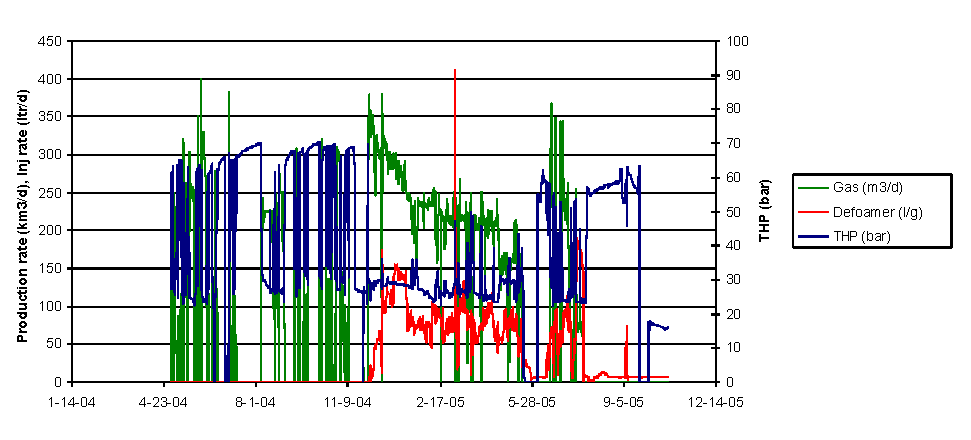
\includegraphics[width=\textwidth]{fig/foamer/continuous-evaluation.eps}
    \caption{Valutazione pre- e post-applicazione di \textit{foamer} in continuo su un pozzo affetto da \textit{liquid loading} \parencite{wittfeld2015foam}.}
    \label{fig:continuous-evaluation}
\end{figure}
Il pozzo era caratterizzato da produzione incostante e veniva aperto solo per brevi periodi. Una volta iniziata l'applicazione di schiumogeno in continuo, la produzione di gas si è notevolmente stabilizzata, con portate medie quasi raddoppiate. Il pozzo ha mantenuto questo andamento e ha garantito produzione di gas per 9 mesi.\\
Alcune sono le condizioni affinché l'applicazione abbia esiti positivi:
\begin{itemize}
    \item \textbf{risposta positiva al \textit{foamer} in-batch}: se un pozzo risponde bene alle applicazioni in-batch, esso può considerarsi un ottimo candidato all'applicazione di schiumogeno in continuo. Questa condizione risulta essere importante ma non necessaria: se un pozzo non reagisce in maniera positiva ai batch di schiuma, non vuol dire in modo assoluto che non sia un candidato idoneo per l'iniezione tramite \textit{capillary string};
    \item \textbf{riduzione sufficiente della portata critica}:  una volta applicato il \textit{foamer} in continuo, il pozzo deve comunque avere sufficiente energia per spiazzare l'acqua e evitare nuovamente l'aumento del battente idrostatico a fondo pozzo. Come già detto all'inizio del paragrafo ~\ref{section:foamer-ll} l'applicazione di \textit{foamer} porta a riduzioni della portata critica fino al 33\%, ciò vuol dire che il pozzo deve avere energia sufficiente a garantire il 66\% della portata critica standard;
    \item \textbf{ottimizzazione del IPR}: è utile stimare le variazioni di IPR dopo l'applicazione del schiumogeno in modo da verificare l'entità della variazione dello stesso parametro. Se la variazione risulta eccessiva, l'installazione della \textit{capillary string} non è particolarmente consigliata;
    \item \textbf{accesso al pozzo}: è necessario che il pozzo non presenti ostacoli o particolari restringimenti per l'installazione della \textit{capillary string} fino alla profondità desiderata;
    \item \textbf{disponibilità a test temporanei}: in alcuni casi, è opportuno condurre un test di 4-5 giorni per verificare l'efficacia del test, il pozzo deve essere quindi predisposto all'installazione anche solo temporanea del sistema di iniezione.
\end{itemize}
I costi legati all'impiego di un sistema di iniezione in continuo sono legati agli investimenti iniziali e ai costi in vita. L'investimento iniziale prevede le modifiche della strumentazione di superficie (~€xxx), l'acquisto della \textit{capillary string} (~€x per metro), la modifica all'SCSSV (~€xxx) e l'installazione della strumentazione in sotterraneo (personale di terra già presente), per una spesa totale di ~€xxxx. I costi in corso di utilizzo sono legati all'impiego di \textit{foamer} e \textit{defoamer} (~€x per litro, quindi ~€xxxx all'anno) e i costi di manutenzione e riparazione (~€xxx), per un totale di ~€xxxx di spese medie annuali.  \\ \\
Non solo gli impianti di produzione, ma anche gli impianti di trattamento del gas risentono notevolmente dei miglioramenti di performance del pozzo: senza dimenticare che l'aumento di portata garantisce maggiori introiti giornalieri, una produzione più regolare consente di trattare il gas in modo più idoneo e sicuro. Per conoscere i vantaggi anche a livello impiantistico, nel prossimo capitolo viene fornito un \textit{excursus} sui trattamenti necessari alla trasportabilità e alla distribuzione del gas naturale